\chapter{Screenshots af SailingClubManager}\label{bilag:scm}

Dette bilag har til formål at underbygge afsnittet "\nameref{chap:teknologi-analyse}  (\ref{chap:teknologi-analyse})". Dette er et system, til administration af både, som vi har fået tilladelse til at prøve af skaberen. Siden hedder SailingClubManager, og er placeret på url'en \href{http://abs.boxstuff.net}{\textit{http://abs.boxstuff.net}}, "abs"\ da vores klub derunder hedder "Aalborg Boat Squad". Det er også muligt at anvende denne service til at lave sin egen hjemmeside til offentligheden, et eksempel på dette er: \href{http://www.thamessailingclub.co.uk/}{\textit{Thames Sailing Club}}.

\begin{figure}
	Siden /boats indholder de både, som er tilføjet af brugeren. \newline
	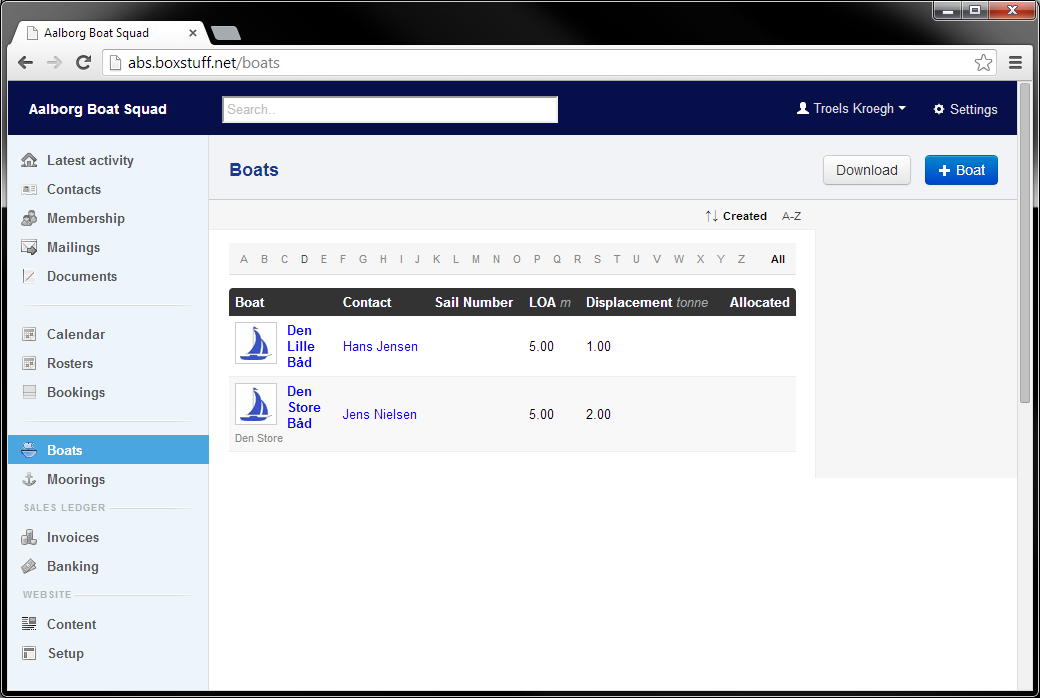
\includegraphics[scale=0.5]{images/teknologi/_Boats}
\end{figure}

\begin{figure}
	Personer som er en del af systemet, er en kontakt. De findes under /contacts.\newline
	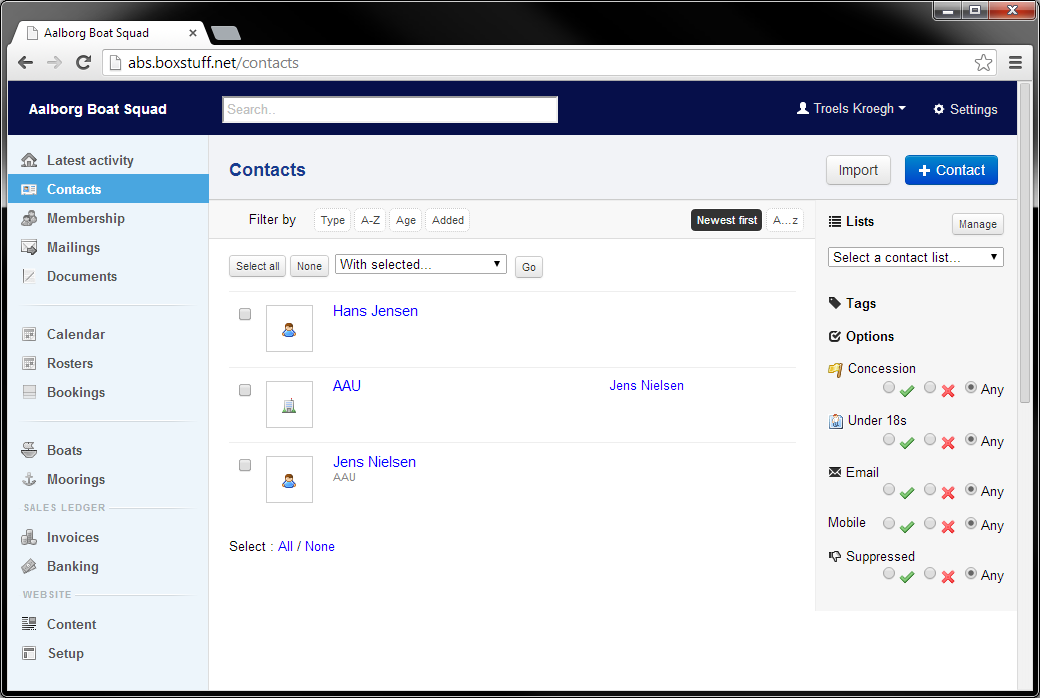
\includegraphics[scale=0.5]{images/teknologi/_Contacts}
\end{figure}

\begin{figure}
	Det er muligt at tilføje nye medlemmer, herunder hvilke type medlem de er. Disse typer er også muligt selv at lave i undermenuen Membership under /memberships/new.\newline
	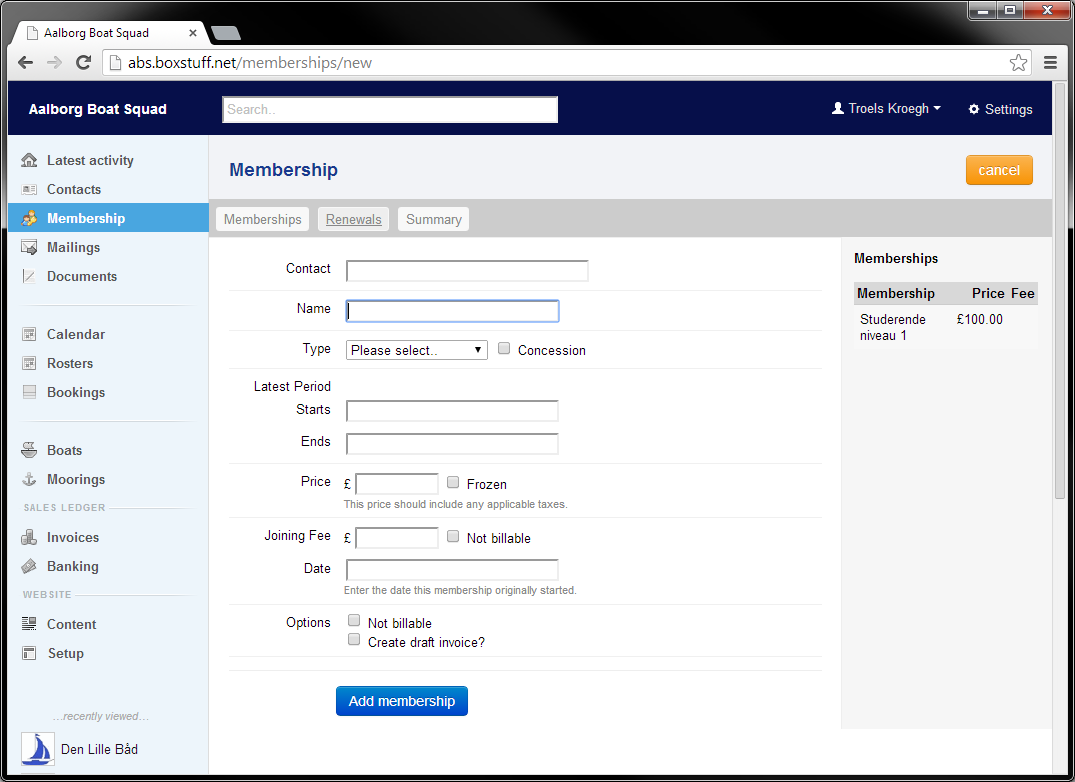
\includegraphics[scale=0.5]{images/teknologi/_AddMember}
\end{figure}

\begin{figure}
	Der findes en kalender med aktiviteter, som administratorer kan tilføje. Under /events.\newline
	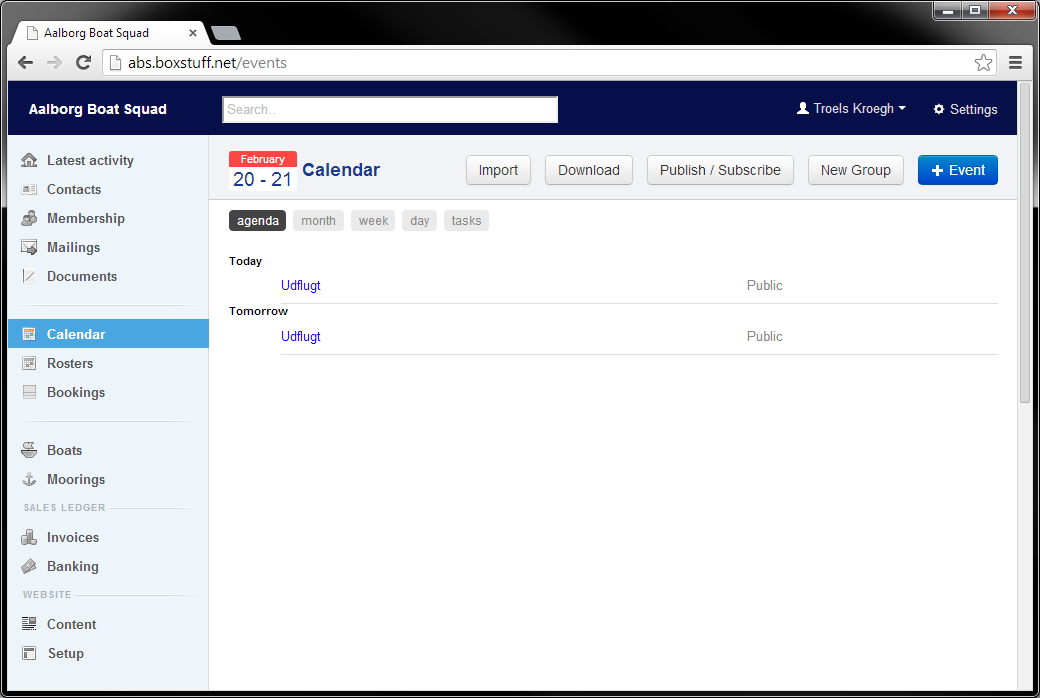
\includegraphics[scale=0.5]{images/teknologi/_Calendar}
\end{figure}

\begin{figure}
	Det er muligt for brugere at booke bådene, her har Hans Jensen booket en båd både den 20-02-2014 og den 26-02-2014. Dette findes under /booking/bookings.\newline
	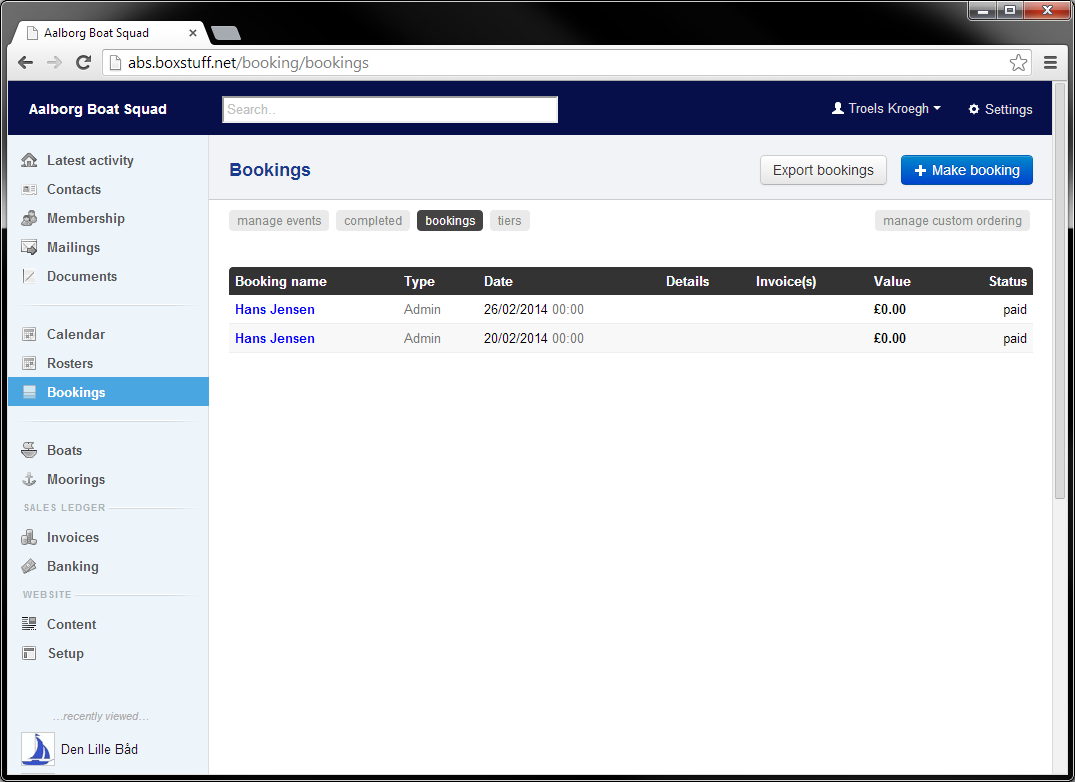
\includegraphics[scale=0.5]{images/teknologi/_Bookings}
\end{figure}

\begin{figure}
	Det er muligt at udskrive regninger baseret på brugeres udlån og kontingent. Under /invoices.\newline
	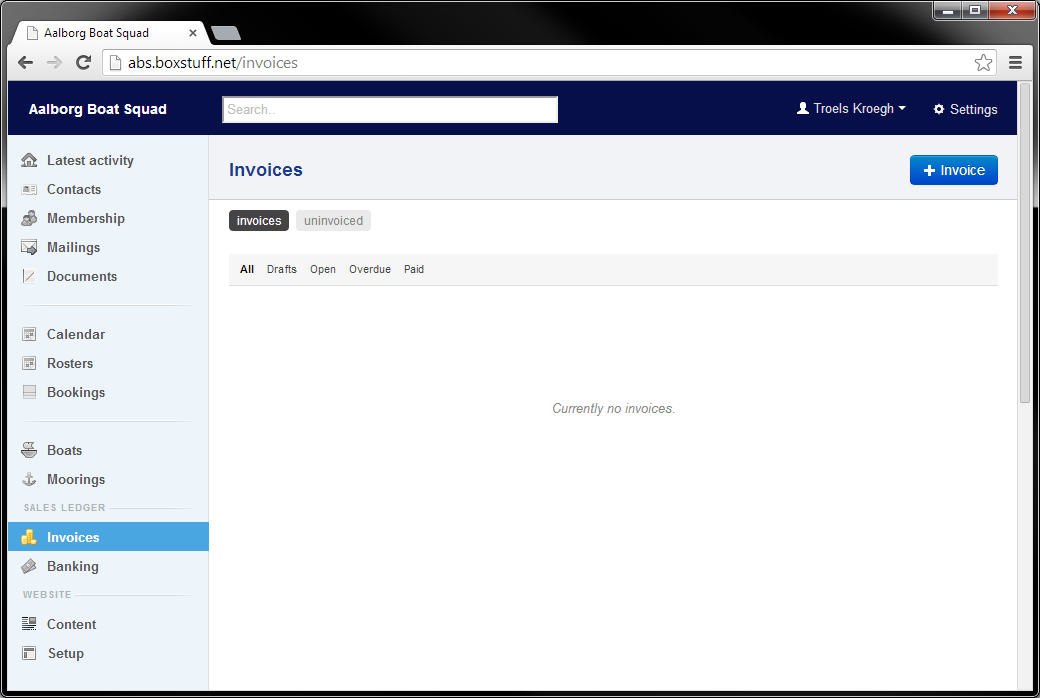
\includegraphics[scale=0.5]{images/teknologi/_Invoices}
\end{figure}
